\UseRawInputEncoding

%%%%%%%%%%%%%%%%%%%%%%%%%%%%%%%%%%%%%%%%%%%%%%%%%%%%%%%%%%%%%%%%%%%%%%%%%%%%%%%%
%% SETTINGS
%%%%%%%%%%%%%%%%%%%%%%%%%%%%%%%%%%%%%%%%%%%%%%%%%%%%%%%%%%%%%%%%%%%%%%%%%%%%%%%%
%% Columns
\documentclass[final,3p,times,twocolumn]{elsarticle}
%% Use the options 1p,twocolumn; 3p; 3p,twocolumn; 5p; or 5p,twocolumn
%% for a journal layout:
%% \documentclass[final,1p,times]{elsarticle}
%% \documentclass[final,1p,times,twocolumn]{elsarticle}
%% \documentclass[final,3p,times]{elsarticle}
%% \documentclass[final,3p,times,twocolumn]{elsarticle}
%% \documentclass[final,5p,times]{elsarticle}
%% \documentclass[final,5p,times,twocolumn]{elsarticle}
%% \documentclass[preprint,review,12pt]{elsarticle}

%% Image width
\newlength{\imagewidth}
\newlength{\imagescale}
%% preamble
\usepackage[english]{babel}
\usepackage[table]{xcolor} % For coloring tables
\usepackage{booktabs} % For professional quality tables
\usepackage{colortbl} % For coloring cells in tables
\usepackage{amsmath, amssymb} % For mathematical symbols and environments
\usepackage{amsthm} % For theorem-like environments
\usepackage{lipsum} % just for sample text
\usepackage{natbib}
\usepackage{graphicx}
\usepackage{indentfirst}
\usepackage{bashful}
\usepackage[margin=10pt,font=small,labelfont=bf,labelsep=endash]{caption}
\usepackage{graphicx}
\usepackage{calc}
\usepackage[T1]{fontenc} % [REVISED]
\usepackage[utf8]{inputenc} % [REVISED]
\usepackage{hyperref}
\usepackage{accsupp}
%% Line numbers
\linespread{1.1}
% \linenumbers
% Tables
\usepackage[pass]{geometry}
\usepackage{pdflscape}
\usepackage{csvsimple}
\usepackage{xltabular}
\usepackage{booktabs}
\usepackage{siunitx}
\usepackage{makecell}
\sisetup{round-mode=figures,round-precision=3}
\renewcommand\theadfont{\bfseries}
\renewcommand\theadalign{c}
\newcolumntype{C}[1]{>{\centering\arraybackslash}m{#1}}
\renewcommand{\arraystretch}{1.5}
\definecolor{lightgray}{gray}{0.95}

%% Diff
\usepackage{xcolor}
% Define commands for highlighting
% diff
\usepackage[most]{tcolorbox} % for boxes with transparency
% Define colors with transparency (opacity value)
\definecolor{GreenBG}{rgb}{0,1,0}
\definecolor{RedBG}{rgb}{1,0,0}
% Define tcolorbox environments for highlighting
\newtcbox{\greenhighlight}[1][]{%
  on line,
  colframe=GreenBG,
  colback=GreenBG!50!white, % 50% transparent green
  boxrule=0pt,
  arc=0pt,
  boxsep=0pt,
  left=1pt,
  right=1pt,
  top=2pt,
  bottom=2pt,
  tcbox raise base
}
\newtcbox{\redhighlight}[1][]{%
  on line,
  colframe=RedBG,
  colback=RedBG!50!white, % 50% transparent red
  boxrule=0pt,
  arc=0pt,
  boxsep=0pt,
  left=1pt,
  right=1pt,
  top=2pt,
  bottom=2pt,
  tcbox raise base
}
\newcommand{\REDSTARTS}{\color{red}}
\newcommand{\REDENDS}{\color{black}}
\newcommand{\GREENSTARTS}{\color{green}}
\newcommand{\GREENENDS}{\color{black}}
%%%%%%%%%%%%%%%%%%%%%%%%%%%%%%%%%%%%%%%%%%%%%%%%%%%%%%%%%%%%%%%%%%%%%%%%%%%%%%%%
%% JOURNAL NAME
%%%%%%%%%%%%%%%%%%%%%%%%%%%%%%%%%%%%%%%%%%%%%%%%%%%%%%%%%%%%%%%%%%%%%%%%%%%%%%%%
\journal{Heliyon}
%%%%%%%%%%%%%%%%%%%%%%%%%%%%%%%%%%%%%%%%%%%%%%%%%%%%%%%%%%%%%%%%%%%%%%%%%%%%%%%%
%% DOCUMENT STARTS
%%%%%%%%%%%%%%%%%%%%%%%%%%%%%%%%%%%%%%%%%%%%%%%%%%%%%%%%%%%%%%%%%%%%%%%%%%%%%%%%
\begin{document}

%%%%%%%%%%%%%%%%%%%%%%%%%%%%%%%%%%%%%%%%%%%%%%%%%%%%%%%%%%%%%%%%%%%%%%%%%%%%%%%%
%% Frontmatter
%%%%%%%%%%%%%%%%%%%%%%%%%%%%%%%%%%%%%%%%%%%%%%%%%%%%%%%%%%%%%%%%%%%%%%%%%%%%%%%%
\begin{frontmatter}
\begin{highlights}
\pdfbookmark[1]{Highlights}{highlights}

\item Neural trajectories in the hippocampus exhibited greater variability during a working memory (WM) task compared to those in the entorhinal cortex and amygdala regions.

\item The distance of neural trajectories between encoding and retrieval states in the hippocampus was memory-load dependent during a WM task.


\item Hippocampal neural trajectories fluctuated between the encoding and retrieval states in a task-dependent manner during both baseline and sharp-wave ripple (SWR) periods.

\item Hippocampal neural trajectories shifted from encoding to retrieval states during SWR period.

\end{highlights}\title{
Hippocampal neural fluctuations between memory encoding and retrieval states during a working memory task in humans
}\author[1]{Yusuke Watanabe\corref{cor1}}
\author[2,3,4]{Yuji Ikegaya}
\author[1,5]{Takufumi Yanagisawa}

\address[1]{Institute for Advanced Cocreation studies, Osaka University, 2-2 Yamadaoka, Suita, 565-0871, Osaka, Japan}
\address[2]{Graduate School of Pharmaceutical Sciences, The University of Tokyo, 7-3-1 Hongo, Tokyo, 113-0033, Japan}
\address[3]{Institute for AI and Beyond, The University of Tokyo, 7-3-1 Hongo, Tokyo, 113-0033, Japan}
\address[4]{Center for Information and Neural Networks, National Institute of Information and Communications Technology, 1-4 Yamadaoka, Suita City, 565-0871, Osaka, Japan}
\address[5]{Department of Neurosurgery, Osaka University Graduate School of Medicine, 2-2 Yamadaoka, Osaka, 565-0871, Japan}

\cortext[cor1]{Corresponding author. Tel: +81-6-6879-3652}%%Graphical abstract
%\pdfbookmark[1]{Graphical Abstract}{graphicalabstract}        
%\begin{graphicalabstract}
%\includegraphics{grabs}
%\end{graphicalabstract}
\begin{abstract}
\pdfbookmark[1]{Abstract}{abstract}
Working memory (WM), critical to various cognitive functions, embodies intricate neural mechanisms which are not entirely understood. Notably, the role of the hippocampus and sharp-wave ripple complexes (SWRs) -- coordinated, rapid neuronal events within the hippocampus -- in WM tasks remains somewhat ambiguous, notwithstanding their confirmed involvement in memory consolidation and retrieval. In our present research, we posit that multiunit activity patterns within the hippocampus operate synergistically with SWRs, consequently exhibiting distinctive dynamics during WM tasks. Our study engaged in a comprehensive analysis of a dataset derived from intracranial electroencephalogram recordings from the medial temporal lobes (MTL) of nine epileptic patients executing an eight-second Sternberg task. Gaussian-process factor analysis was utilized to pinpoint low-dimensional neural vectors, or 'trajectories,' within the MTL during the WM task. We discovered that the hippocampus showed the most pronounced variation in neural trajectories relative to the entorhinal cortex and the amygdala. Intriguingly, the deviation in trajectories between the encoding and retrieval phases was seen to be dependent on memory load. Further, hippocampal trajectories showed oscillatory behavior during the retrieval phase, indicating task-related transitions between encoding and retrieval states, and embracing both baseline and SWR episodes. These oscillations transitioned from encoding to retrieval states in correlation with the SWRs. Hence, these findings underscore the crucial role of the hippocampus in tackling WM tasks and propose an enticing hypothesis for future exploration: the functional state of the hippocampus switches from encoding to retrieval during SWRs.
\end{abstract}% \pdfbookmark[1]{Keywords}{keywords}                
\begin{keyword}
working memory \sep WM \sep memory load \sep hippocampus \sep sharp-wave ripples \sep SWR \sep humans
\end{keyword}
\end{frontmatter}

%%%%%%%%%%%%%%%%%%%%%%%%%%%%%%%%%%%%%%%%%%%%%%%%%%%%%%%%%%%%%%%%%%%%%%%%%%%%%%%%
%% IMRaD
%%%%%%%%%%%%%%%%%%%%%%%%%%%%%%%%%%%%%%%%%%%%%%%%%%%%%%%%%%%%%%%%%%%%%%%%%%%%%%%%

%%%%%%%%%%%%%%%%%%%%%%%%%%%%%%%%%%%%%%%%%%%%%%%%%%%%%%%%%%%%%%%%%%%%%%%%%%%%%%%%
%% INTRODUCTION
%%%%%%%%%%%%%%%%%%%%%%%%%%%%%%%%%%%%%%%%%%%%%%%%%%%%%%%%%%%%%%%%%%%%%%%%%%%%%%%%
Working memory (WM) serves a critical role in everyday life, with its neural foundations being an ongoing subject of study. The hippocampus, particularly crucial to memory function, remains central to this research \cite{scoville_loss_1957} \cite{squire_legacy_2009}  \cite{boran_persistent_2019} \cite{kaminski_persistently_2017} \cite{kornblith_persistent_2017} \cite{faraut_dataset_2018} \cite{borders_hippocampus_2022} \cite{li_functional_2023} \cite{dimakopoulos_information_2022}. Understanding the role of the hippocampus in working memory is essential to advancing our comprehension of cognitive processes, thereby promoting cognitive training and interventions.
\\
\indent
Current evidence points toward a brief, synchronized oscillation, known as sharp-wave ripple (SWR) \cite{buzsaki_hippocampal_2015}, being associated with several cognitive functions. These include memory replay \cite{wilson_reactivation_1994} \cite{nadasdy_replay_1999} \cite{lee_memory_2002} \cite{diba_forward_2007} \cite{davidson_hippocampal_2009}, memory consolidation \cite{girardeau_selective_2009} \cite{ego-stengel_disruption_2010} \cite{fernandez-ruiz_long-duration_2019} \cite{kim_corticalhippocampal_2022}, memory recall \cite{wu_hippocampal_2017} \cite{norman_hippocampal_2019} \cite{norman_hippocampal_2021}, and neural plasticity \cite{behrens_induction_2005} \cite{norimoto_hippocampal_2018}. This suggests that SWR may play a crucial part in hippocampal processing, contributing to the performance of working memory. However, studies investigating the effects of SWRs on working memory are limited \cite{jadhav_awake_2012} and focus primarily on rodent models engaged in navigation tasks, without clear delineation of memory acquisition and recall timing.
\\
\indent
Recent studies have illustrated that hippocampal neurons present low-dimensional representations during WM tasks. Specifically, the firing patterns of place cells \cite{okeefe_hippocampus_1971} \cite{okeefe_place_1976} \cite{ekstrom_cellular_2003} \cite{kjelstrup_finite_2008} \cite{harvey_intracellular_2009}, located in the hippocampus, appear within a dynamic, nonlinear three-dimensional hyperbolic geometry in rodent models \cite{zhang_hippocampal_2022}. Additionally, grid cells in the entorhinal cortex (EC)—the main route to the hippocampus \cite{naber_reciprocal_2001} \cite{van_strien_anatomy_2009} \cite{strange_functional_2014}—display a toroidal topology during exploration \cite{gardner_toroidal_2022}. Regrettably, these studies are limited to spatial navigation tasks in rodents, affecting the temporal resolution of WM tasks. The application of these findings to human subjects and their extension beyond navigation tasks are still unconfirmed.
\\
\indent
In light of these points, the present study seeks to corroborate the hypothesis that hippocampal neurons portray unique representations in low-dimensional spaces, referred to as 'neural trajectory,' particularly during SWR periods in WM tasks. To test this proposition, we used a dataset from patients performing an eight-second Sternberg task (1 second for fixation, 2 seconds for encoding, 3 seconds for maintenance, and 2 seconds for retrieval) with a high temporal resolution, while their intracranial electroencephalography (iEEG) signals in the medial temporal lobe (MTL) were monitored \cite{boran_dataset_2020}. To explore the low-dimensional neural trajectories, we utilized the Gaussian-process factor analysis (GPFA), a recognized technique for examining neural population dynamics \cite{yu_gaussian-process_2009}.
\label{sec:introduction}
%%%%%%%%%%%%%%%%%%%%%%%%%%%%%%%%%%%%%%%%%%%%%%%%%%%%%%%%%%%%%%%%%%%%%%%%%%%%%%%%
%% METHODS
%%%%%%%%%%%%%%%%%%%%%%%%%%%%%%%%%%%%%%%%%%%%%%%%%%%%%%%%%%%%%%%%%%%%%%%%%%%%%%%%
\section{Methods}
\subsection{Dataset}
A public dataset \cite{boran_dataset_2020} comprising experiments from nine epilepsy patients was taken into consideration for this study. The patients were tasked with executing a modified Sternberg task which included four phases: fixation (1s), encoding (2s), maintenance (3s), and retrieval (2s) \cite{boran_dataset_2020}. During the encoding phase, participants were presented with four, six, or eight alphabet letters, known as the set size. Subsequently, they had to ascertain whether a probe letter revealed during the retrieval phase was displayed earlier (the suitable choice for the Match IN task) or not (the suitable choice for the Mismatch OUT task). iEEG signals were registered via a sampling rate of 32 kHz, within a frequency spectrum of 0.5--5,000 Hz, utilizing depth electrodes implanted in the medial temporal lobe (MTL) regions: the anterior head of the left and right hippocampus (AHL and AHR), the posterior body of the hippocampus (PHL and PHR), the entorhinal cortex (ECL and ECR), and the amygdala (AL and AR) (Figure~\ref{fig:01}A and Table~\ref{tab:01}). The recorded iEEG signals were subsequently downsampled to a rate of 2 kHz. The interrelationship among variables such as set size and correct rate were explored (Figure~\ref{fig:s01}S1). The timings of multiunit spikes were identified using a spike sorting algorithm \cite{niediek_reliable_2016} with the Combinato package (\url{https://github.com/jniediek/combinato}) (Figure~\ref{fig:01}C).

\subsection{Calculation of neural trajectories using GPFA}
Neural trajectories, colloquially called 'factors' (Figure~\ref{fig:01}D), in the hippocampus, EC, and amygdala (Figure~\ref{fig:01}D) were calculated utilizing GPFA \cite{yu_gaussian-process_2009}, which was applied to the multiunit activity data radiating from each session. The computations were performed with the elephant package (\url{https://elephant.readthedocs.io/en/latest/reference/gpfa.html}). The bin size was set at 50 ms, with no overlaps. Each factor was z-normalized across all sessions. The Euclidean distance from the origin ($O$) was subsequently calculated (Figure~\ref{fig:01}E).
\\
\indent
For each trajectory inside a region, for example, AHL, \textit{geometric medians} ($\mathrm{g_{F}}$ for fixation, $\mathrm{g_{E}}$ for encoding, $\mathrm{g_{M}}$ for maintenance, and $\mathrm{g_{R}}$ for retrieval phase) were calculated by finding the median coordinates of the trajectory during the four phases (Figure~\ref{fig:01}D). An optimal dimensionality for GPFA was identified as three using the elbow method, which was derived by investigating the log-likelihood values through a three-fold cross-validation technique (Figure~\ref{fig:02}B).

\subsection{Identifying SWR candidates from areas of the hippocampus}
Potential SWR instances from within the hippocampus were identified via an accepted method \cite{liu_consensus_2022}. LFP signals from a given region of interest (ROI), such as AHL, were re-referenced by subtracting a calculated average signal from locations outside the ROI (e.g., AHR, PHL, PHR, ECL, ECR, AL, and AR) (see Figure~\ref{fig:01}A). The re-referenced LFP signals were further filtered with a ripple-band filter (80--140 Hz) to detect SWR candidates (=$\textrm{SWR}^+$ candidates) (see Figure~\ref{fig:01}B). SWR detection was carried out using a published tool (\url{https://github.com/Eden-Kramer-Lab/ripple_detection}) \cite{kay_hippocampal_2016}, with the bandpass range adjusted to 80--140 Hz in line with human requirements \cite{norman_hippocampal_2019} \cite{norman_hippocampal_2021}, as opposed to the conventional 150--250 Hz range typically applied to rodents.
\\
\indent
Control events for $\textrm{SWR}^+$ candidates, tagged as $\textrm{SWR}^-$ candidates, were identified by shuffling the timestamps of $\textrm{SWR}^+$ candidates randomly across all trials and subjects. The resultant $\textrm{SWR}^+/\textrm{SWR}^-$ candidates underwent visual inspection (Figure~\ref{fig:01}).

\subsection{Defining SWRs from alleged hippocampal CA1 regions}
SWRs were distinguished from SWR candidates within likely CA1 regions. Initially, these regions were designated as follows: $\textrm{SWR}^+/\textrm{SWR}^-$ candidates from the hippocampus were mapped into a two-dimensional space based on the overlapping spike counts per unit using a supervised UMAP (Uniform Manifold Approximation and Projection) \cite{mcinnes_umap_2018} (Figure~\ref{fig:04}A). Validation of the clustering was done by computing the silhouette score \cite{rousseeuw_silhouettes_1987} from the clustered samples (Table~\ref{tab:02}). Those areas in the hippocampus scoring over 0.6 on average across sessions (or the 75th percentile) were specified as likely CA1 regions, in turn, identifying five electrode positions across five participants (Table~\ref{tab:03}).
\\
\indent
Those $\textrm{SWR}^+/\textrm{SWR}^-$ candidates within the assumed CA1 regions were classified as $\textrm{SWR}^+/\textrm{SWR}^-$ and had their candidate status revoked. Log-normal distributions were observed in the duration and ripple band peak amplitude of SWRs (Figure~\ref{fig:04}4C & E). Each SWR time period was partitioned relative to the time from the SWR center into pre- (at $-800$ to $-300$ ms from SWR center), mid- (at $-250$ to $+250$ ms), and post- (at $+300$ to $+800$ ms) SWR times.

\subsection{Statistical evaluation}
The Brunner--Munzel test and the Kruskal-Wallis test were performed using the SciPy package in Python \cite{virtanen_scipy_2020}. A correlation analysis was executed by determining the rank of the correlation coefficient in its associated set-size-shuffled surrogate using a custom Python script. The bootstrap test was conducted with an in-house Python script.

\label{sec:methods}
%%%%%%%%%%%%%%%%%%%%%%%%%%%%%%%%%%%%%%%%%%%%%%%%%%%%%%%%%%%%%%%%%%%%%%%%%%%%%%%%
%% RESULTS
%%%%%%%%%%%%%%%%%%%%%%%%%%%%%%%%%%%%%%%%%%%%%%%%%%%%%%%%%%%%%%%%%%%%%%%%%%%%%%%%
\section{Results}
\subsection{iEEG recording and neural trajectory in MTL regions during a Sternberg task}
We analyzed a publicly available dataset for this study \cite{boran_dataset_2020}. This dataset consists of LFP signals (Figure 1A) from MTL regions (Table~\ref{tab:01}) obtained during a modified Sternberg task performance. We identified SWR$^+$ candidates from LFP signals filtered through the 80--140 Hz ripple band (Figure 1B) across all hippocampal regions (refer to Methods). Correspondingly, SWR$^-$ candidates were defined at the same timestamps but shuffled between different trials (Figure 1). The dataset included multiunit spikes (Figure 1C) identified via a spike sorting algorithm \cite{niediek_reliable_2016}. Using GPFA \cite{yu_gaussian-process_2009}, and 50-ms binned multiunit activity without overlaps, we determined the neural trajectories (or factors) of MTL regions per session and region (Figure 1D). We normalized each factor by session and region, for instance, session \#2 in AHL of subject \#1. Subsequently, we calculated the Euclidean distance from the origin ($O$) (Figure 1E).

\subsection{Correlation between hippocampal neural trajectory and Sternberg task performance}
Figure 2A shows the cloud of median neural trajectories of 50 trials within the three main factor spaces. We determined the optimal embedding dimension for the GPFA model to be three, using the elbow method (Figure 2B). The trajectory distance from the origin ($O$) (represented as $\mathrm{\lVert g_{F} \rVert}$, $\mathrm{\lVert g_{E} \rVert}$, $\mathrm{\lVert g_{M} \rVert}$, and $\mathrm{\lVert g_{R} \rVert}$) in the hippocampus was greater than the corresponding distances in the EC and amygdala (Figures 2C and D).\footnote{Hippocampus: Distance = 1.11 [1.01], median [IQR], \textit{n} = 195,681 timepoints; EC: Distance = 0.94 [1.10], median [IQR], \textit{n} = 133,761 timepoints; Amygdala: Distance = 0.78 [0.88], median [IQR], \textit{n} = 165,281 timepoints.}
\\
\indent
Similarly, we calculated the distances between the geometric medians of the four phases, namely $\mathrm{\lVert g_{F}g_{E} \rVert}$, $\mathrm{\lVert g_{F}g_{M} \rVert}$, $\mathrm{\lVert g_{F}g_{R} \rVert}$, $\mathrm{\lVert g_{E}g_{M} \rVert}$, $\mathrm{\lVert g_{E}g_{R} \rVert}$, and $\mathrm{\lVert g_{M}g_{R} \rVert}$. The results indicated that the hippocampus showed larger distances between phases than both the EC and amygdala. \footnote{Hippocampus: Distance = 0.60 [0.70], median [IQR], \textit{n} = 8,772 combinations; EC: Distance = 0.28 [0.52], median [IQR], \textit{n} = 5,017 combinations (\textit{p} $<$ 0.01; Brunner--Munzel test); Amygdala: Distance = 0.24 [0.42], median [IQR], \textit{n} = 7,466 combinations (\textit{p} $<$ 0.01; Brunner--Munzel test).}

\subsection{Memory load-dependence of neural trajectory distance between encoding and retrieval states in the hippocampus}
In the context of memory load in the Sternberg task, we found a negative correlation between the correct rate of trials and set size (the number of letters to encode) (Figure 3A).\footnote{Correct rate: set size four (0.99 \textpm 0.11, mean \textpm SD; \textit{n} = 333 trials) vs. set size six (0.93 \textpm 0.26; \textit{n} = 278 trials; \textit{p} $<$ 0.001, Brunner--Munzel test with Bonferroni correction) and set size eight (0.87 \textpm 0.34; \textit{n} = 275 trials; \textit{p} $<$ 0.05; Brunner--Munzel test with Bonferroni correction). Overall, \textit{p} $<$ 0.001 for Kruskal--Wallis test; correlation coefficient = - 0.20, \textit{p} $<$ 0.001.} Similarly, we observed a positive correlation between the response time and set size (Figure 3B).\footnote{Response time: set size four (1.26 \textpm 0.45 s; \textit{n} = 333 trials) vs. set size six (1.53 \textpm 0.91 s; \textit{n} = 278 trials) and set size eight (1.66 \textpm 0.80 s; \textit{n} = 275 trials). All comparisons \textit{p} $<$ 0.001, Brunner--Munzel test with Bonferroni correction; \textit{p} $<$ 0.001 for Kruskal--Wallis test; correlation coefficient = 0.22, \textit{p} $<$ 0.001}.
\\
\indent
Additionally, we observed a positive correlation between set size and the trajectory distance between the encoding and retrieval phases ($\mathrm{log_{10}\lVert g_{E}g_{R} \rVert}$) (Figure 3C).\footnote{Correlation between set size and $\mathrm{log_{10}(\lVert g_{E}g_{R} \rVert}$): correlation coefficient = 0.05, \textit{p} $<$ 0.001. Specific values: $\mathrm{\lVert g_{E}g_{R} \rVert}$ = 0.54 [0.70] for set size four, \textit{n} = 447; $\mathrm{\lVert g_{E}g_{R} \rVert}$ = 0.58 [0.66] for set size six, \textit{n} = 381; $\mathrm{\lVert g_{E}g_{R} \rVert}$ = 0.61 [0.63] for set size eight, \textit{n} = 395.}. However, the distances between other combinations of phases did not show significant correlations (Figures 3D and S2).

\subsection{Detection of hippocampal SWR from putative CA1 regions}
To better localize recording sites and improve SWR detection, we estimated the electrode position in the CA1 regions of the hippocampus using distinct multiunit spike patterns during SWR events. We embedded SWR$^+$/SWR$^-$ candidates from each session and hippocampal region in a two-dimensional space via UMAP (Figure 4A).\footnote{Consider the AHL in session \#1 of subject \#1, for illustration purposes.} The quality of clustering was verified using the silhouette score as a metric (Figure 4B and Table~\ref{tab:02}). Recording sites yielding an average silhouette score over 0.6 across all sessions were designated as putative CA1 regions.\footnote{The designated regions were: AHL of subject \#1, AHR of subject \#3, PHL of subject \#4, AHL of subject \#6, and AHR of subject \#9.} (Tables~\ref{tab:02} and \ref{tab:03}). We found five putative CA1 regions, out of which four weren't labeled as seizure onset zones (Table~\ref{tab:01}).
\\
\indent
We further labeled SWR$^+$/SWR$^-$ candidates within these putative CA1 regions as SWR$^+$ and SWR$^-$, respectively\footnote{These definitions resulted in equal counts for both categories: SWR$^+$ (\textit{n} = 1,170) and SWR$^-$ (\textit{n} = 1,170).}  (Table~\ref{tab:03}). Both SWR$^+$ and SWR$^-$ exhibited equal duration\footnote{These definitions resulted in equal durations for both categories: SWR$^+$ (93.0 [65.4] ms) and SWR$^-$ (93.0 [65.4] ms).}   (Figure 4C) due to their definitions, and adopted a log-distribution. There was an increase in SWR$^+$ incidence within the first 400 ms of the retrieval phase\footnote{The occurrence of SWR$^+$ increased against the bootstrap sample; 95th percentile = 0.42 [Hz]; \textit{p} $<$ 0.05.}  (Figure 4D). The peak ripple band amplitude of SWR$^+$ was greater than that of SWR$^-$ and followed a log-normal distribution (Figure 4E).\footnote{SWR$^+$ (3.05 [0.85] SD of baseline, median [IQR]; \textit{n} = 1,170) vs. SWR$^-$ (2.37 [0.33] SD of baseline, median [IQR]; \textit{n} = 1,170; \textit{p} $<$ 0.001; Brunner--Munzel test).}.

\subsection{Transient changes in hippocampal neural trajectories during SWR events}
We calculated the distance of the trajectory from the origin ($O$) during SWR events in both the encoding and retrieval phases (Figure 5A). Observing an increase in distance during SWR as shown in Figure 5A, we classified each SWR into three stages: pre-, mid-, and post-SWR. Consequently, the distances from $O$ during these SWR stages are denoted as $\mathrm{\lVert \text{pre-eSWR}^+ \rVert}$, $\mathrm{\lVert \text{mid-eSWR}^+ \rVert}$ among others.
\\
\indent
The $\mathrm{\lVert \text{mid-eSWR}^+ \rVert}$\footnote{1.25 [1.30], median [IQR], \textit{n} = 1,281, in Match IN task; 1.12 [1.35], median [IQR], \textit{n} = 1,163, in Mismatch OUT task} was larger than $\mathrm{\lVert \text{pre-eSWR}^+ \rVert}$\footnote{1.08 [1.07], median [IQR], \textit{n} = 1,149, in Match IN task; 0.90 [1.12], median [IQR], \textit{n} = 1,088, in Mismatch OUT task}, and $\mathrm{\lVert \text{mid-rSWR}^+ \rVert}$\footnote{1.32 [1.24], median [IQR], \textit{n} = 935, in Match IN task; 1.15 [1.26], median [IQR], \textit{n} = 891, in Mismatch OUT task} was bigger than $\mathrm{\lVert \text{pre-rSWR}^+ \rVert}$ in both Match IN and Mismatch OUT tasks.\footnote{1.19 [0.96], median [IQR], \textit{n} = 673, in Match IN task; 0.94 [0.88], median [IQR], \textit{n} = 664, in Mismatch OUT task}.

\subsection{Visualization of hippocampal neural trajectories during SWR in two-dimensional spaces}
Following our observations on neural trajectory 'jumping' during a SWR event (Figure 5), we visualized the three-dimensional trajectories of pre-, mid-, and post-SWR events during the encoding and retrieval phases (Figure 6), the distance between which was found to depend on memory load (Figure 3).
\\
\indent
To enable two-dimensional visualization, we linearly aligned peri-SWR trajectories by assigning $\mathrm{g_{E}}$ at the origin (0, 0) and $\mathrm{g_{R}}$ at ($\mathrm{\lVert g_{E}g_{R} \rVert}$, 0). We then rotated these aligned trajectories around the $\mathrm{g_{E}g_{R}}$ axis (the x-axis). This method ensured that the distances from the origin in the original three-dimensional spaces were preserved in the two-dimensional counterparts.
\\
\indent
The scatter plot within these two-dimensional spaces illustrate characteristic distributions of peri-SWR trajectories based on the phases and types of task. One can observe, for example, that the magnitude of  $\mathrm{\lVert \text{mid-eSWR}^+ \rVert}$ surpasses that of $\mathrm{\lVert \text{pre-eSWR}^+ \rVert}$ (Figure 6B), which is consistent with our earlier findings (Figure 5).

\subsection{Directionality of hippocampal neural trajectories between encoding and retrieval states}
We then investigated the \textit{directions} of the trajectories in relation to $\overrightarrow{\mathrm{g_{E}g_{R}}}$. The directions of SWRs were defined by the neural trajectory at $-250$ ms and $+250$ ms from their center, namely $\overrightarrow{\mathrm{eSWR^+}}$.
\\
\indent
We calculated the density of $\overrightarrow{\mathrm{eSWR}} \cdot \overrightarrow{\mathrm{g_{E}g_{R}}}$, $\overrightarrow{\mathrm{rSWR}} \cdot \overrightarrow{\mathrm{g_{E}g_{R}}}$, and $\overrightarrow{\mathrm{eSWR}} \cdot \overrightarrow{\mathrm{rSWR}}$ (Figures 7A--D). The $\overrightarrow{\mathrm{rSWR^-}} \cdot \overrightarrow{\mathrm{g_{E}g_{R}}}$ demonstrated a biphasic distribution.
\\
\indent
By comparing the distribution of $\overrightarrow{\mathrm{rSWR^+}} \cdot \overrightarrow{\mathrm{g_{E}g_{R}}}$ (Figures 7A and B) with that of $\overrightarrow{\mathrm{rSWR^-}} \cdot \overrightarrow{\mathrm{g_{E}g_{R}}}$ (Figures 7C and D), we computed the contributions of SWR (Figures 7E and F), which indicated a shift in the direction of $\overrightarrow{\mathrm{g_{E}g_{R}}}$ (Figures 7E and F: \textit{red rectangles}).
\\
\indent
Furthermore, and only in the Mismatch OUT task, $\overrightarrow{\mathrm{eSWR^+}} \cdot \overrightarrow{\mathrm{rSWR^+}}$ was less than $\overrightarrow{\mathrm{eSWR^-}} \cdot \overrightarrow{\mathrm{rSWR^-}}$ (baseline periods) (Figure 7F: \textit{pink circles}). Put simply, eSWR and rSWR pointed in opposite directions only in the Mismatch OUT task but not in the Match IN task (Figure 7E: \textit{pink circles}).
\label{sec:results}\section{Discussion}
%%%%%%%%%%%%%%%%%%%%%%%%%%%%%%%%%%%%%%%%%%%%%%%%%%%%%%%%%%%%%%%%%%%%%%%%%%%%%%%%
%% DISCUSSION
%%%%%%%%%%%%%%%%%%%%%%%%%%%%%%%%%%%%%%%%%%%%%%%%%%%%%%%%%%%%%%%%%%%%%%%%%%%%%%%%
\section{Discussion}
This study posits that hippocampal neurons generate distinct trajectories within low-dimensional spaces during a working memory (WM) task in humans, specifically during sharp-wave ripple (SWR) periods. Initially, multiunit spikes in the medial temporal lobe (MTL) regions were projected onto three-dimensional spaces during a Sternberg task using Gaussian Process Factor Analysis (GPFA) (Figure~\ref{fig:01}D--E and Figure~\ref{fig:02}A). The trajectory distance across WM phases ($\mathrm{\lVert g_{F}g_{E} \rVert}$, $\mathrm{\lVert g_{F}g_{M} \rVert}$, $\mathrm{\lVert g_{F}g_{R} \rVert}$, $\mathrm{\lVert g_{E}g_{M} \rVert}$, $\mathrm{\lVert g_{E}g_{R} \rVert}$, and $\mathrm{\lVert g_{M}g_{R} \rVert}$) was markedly larger in the hippocampus than in the EC and amygdala (Figure~\ref{fig:02}E), which implies dynamic neural activity in the hippocampus during the WM task. Additionally, in the hippocampus, the trajectory distance between encoding and retrieval phases ($\mathrm{\lVert g_{F}g_{E} \rVert}$) was found to positively correlate with memory load (Figure~\ref{fig:03}C--D), denoting WM processing. The hippocampal neural trajectory momentarily increased during SWRs (Figure~\ref{fig:05}). Eventually, the hippocampal neural trajectory alternated between encoding and retrieval states, progressing specifically from encoding to retrieval during SWR events (Figure~\ref{fig:07}). Such discoveries not only interpret varying aspects of hippocampal neural activity during a WM task in humans, but also offer fresh insights into how SWRs help alter neural states.

Our findings show that the distance of hippocampal neural trajectory across the phases, even after considering the distance from $O$ in these regions, surpassed that in the EC and amygdala (Figure~\ref{fig:02}C--E). This reaffirms the participation of the hippocampus in the WM task, coinciding with prior assertions of hippocampal persistent firing during the maintenance phase \cite{boran_persistent_2019} \cite{kaminski_persistently_2017} \cite{kornblith_persistent_2017} \cite{faraut_dataset_2018}. However, when applying GPFA to multiunit activity during a 1-second level resolution of the WM task, we noticed that the neural trajectory in low-dimensional space demonstrated a memory-load dependence between encoding and retrieval phases, denoted as $\mathrm{\lVert g_{E}g_{R} \rVert}$ (Figure~\ref{fig:03}). This supports the association between the hippocampus and WM processing.

Our analysis focused on putative CA1 regions (Figure~\ref{fig:04}), which is supported by various contributions. This specific concentration arises from well-established observations where SWRs coincide with spike clusters of interneurons and pyramidal neurons \cite{buzsaki_two-stage_1989} \cite{quyen_cell_2008} \cite{royer_control_2012} \cite{hajos_input-output_2013}, potentially within a 50 $\mu$m radius of the recording site \cite{schomburg_spiking_2012}. An increase in the instances of SWRs was identified during the first 0--400 ms of the retrieval phase (Figure~\ref{fig:04}D). This observation aligns with earlier reports of increased SWR occurrence before spontaneous verbal recall \cite{norman_hippocampal_2019} \cite{norman_hippocampal_2021}, reinforcing our findings under a triggered retrieval condition. The log-normal distributions of both SWR length and ripple band peak amplitude observed in this study (Figure~\ref{fig:04}C \& E) concur with the field's consensus \cite{liu_consensus_2022}. Consequently, confining recordings to putative CA1 regions likely improved the accuracy of SWR detection. However, the observed increase in trajectory distance from $O$ during SWRs (Figure~\ref{fig:05}) may be skewed higher due to channel selection. Nevertheless, this potential bias does not significantly undermine our primary conclusions.

Interestingly, during the retrieval phase, trajectory directions alternated between encoding and retrieval states both during baseline and SWR periods (Figure~\ref{fig:07}C \& D). Furthermore, the balance of this oscillation transitioned from encoding to retrieval state during SWR episodes (Figure~\ref{fig:07} E \& F). These outcomes align with preceding reports regarding the role of SWRs in memory retrieval \cite{norman_hippocampal_2019} \cite{norman_hippocampal_2021}. Our findings suggest a novel understanding where SWRs occur when the hippocampal representation transitions from encoding to retrieval states, thereby revealing unexplored aspects of hippocampal representations, such as (i) neuronal oscillation between encoding and retrieval phases during a WM task, and (ii) SWR functioning as a catalyst for changing neural states.

Moreover, our study identified differences between encoding- and retrieval-SWRs (Figure~\ref{fig:07}E--F) specific to WM-task types. Notably, counter movements of encoding-SWR (eSWR) and retrieval-SWR (rSWR) were not seen in the Match IN task but were evident in the Mismatch OUT task. The memory engram theory can explain these observations \cite{liu_optogenetic_2012}. The Match In task, for instance, presented participants with previous letters, whereas the Mismatch OUT task introduced a new letter absent in the encoding phase. These interpretations highlight the vital role of SWR in human cognitive processes.

In conclusion, this investigation demonstrated that during a WM task, hippocampal activity oscillates between encoding and retrieval states, uniquely transitioning from encoding to retrieval during SWR events. These findings offer valuable insights into the neural substrates and workings of working memory within the hippocampus.
\label{sec:discussion}

%%%%%%%%%%%%%%%%%%%%%%%%%%%%%%%%%%%%%%%%%%%%%%%%%%%%%%%%%%%%%%%%%%%%%%%%%%%%%%%%
%% REFERENCE STYLES
%%%%%%%%%%%%%%%%%%%%%%%%%%%%%%%%%%%%%%%%%%%%%%%%%%%%%%%%%%%%%%%%%%%%%%%%%%%%%%%%
\pdfbookmark[1]{References}{references}
\bibliography{bibliography}
% Note Re-compile is required

%% Numbering Style (sorted)
\bibliographystyle{elsarticle-num}

% Author Style
% \bibliographystyle{plainnat}
% use \citet{}

%% Numbering Style (not-sorted) 
% \bibliographystyle{plainnat}
% use \cite{}



%%%%%%%%%%%%%%%%%%%%%%%%%%%%%%%%%%%%%%%%%%%%%%%%%%%%%%%%%%%%%%%%%%%%%%%%%%%%%%%%
%% ADDITIONAL INFORMATION
%%%%%%%%%%%%%%%%%%%%%%%%%%%%%%%%%%%%%%%%%%%%%%%%%%%%%%%%%%%%%%%%%%%%%%%%%%%%%%%%
\pdfbookmark[1]{Additional Information}{additional_information}

\pdfbookmark[2]{Contributors}{contributors}                    
\section*{Contributors}
Y.W. and T.Y. conceptualized the study; Y.W. performed the data analysis; Y.W. and T.Y. wrote the original draft; and all authors reviewed the final manuscript.
\label{contributors}

\pdfbookmark[2]{Acknowledgments}{acknowledgments}                    
\section*{Acknowledgments}
This research was funded by a grant from the Exploratory Research for Advanced Technology (JPMJER1801).
\label{acknowledgments}

\pdfbookmark[2]{Declaration of Interests}{declaration_of_interest}                    
\section*{Declaration of Interests}
The authors declare that they have no competing interests.
\label{declaration of interests}

\pdfbookmark[2]{Data and code availability}{data_and_code_availability}                    
\section*{Data and code availability}
The data is available on G-Node (\url{https://doi.gin.g-node.org/10.12751/g-node.d76994/}). The source code is available on GitHub (\url{https://github.com/yanagisawa-lab/hippocampal-neural-fluctuation-during-a-WM-task-in-humans}).
\label{data and code availability}

\pdfbookmark[2]{Inclusion and Diversity Statement}{inclusion_and_diversity_statement}        
\section*{Inclusion and Diversity Statement}
We support inclusive, diverse, and equitable conduct of research.
\label{inclusion and diversity statement}

\pdfbookmark[2]{Declaration of Generative AI in Scientific Writing}{declaration_of_generative_ai}
\section*{Declaration of Generative AI in Scientific Writing}
The authors employed ChatGPT, provided by OpenAI, for enhancing the manuscript's English language quality. After incorporating the suggested improvements, the authors meticulously revised the content. Ultimate responsibility for the final content of this publication rests entirely with the authors.
\label{declaration of generative ai in scientific writing}

%% \pdfbookmark[2]{Appendices}{appendices}                    
%% \appendix
%% \section{}
%% \label{}

%%%%%%%%%%%%%%%%%%%%%%%%%%%%%%%%%%%%%%%%%%%%%%%%%%%%%%%%%%%%%%%%%%%%%%%%%%%%%%%%
%% TABLES
%%%%%%%%%%%%%%%%%%%%%%%%%%%%%%%%%%%%%%%%%%%%%%%%%%%%%%%%%%%%%%%%%%%%%%%%%%%%%%%%
\clearpage
\section*{Tables}
\label{tables}
\pdfbookmark[1]{Tables}{tables}
\pdfbookmark[2]{ID 01}{id_01}
\begin{table*}[htbp]
\centering
\small
\begin{tabular}{*{11}{c}}
\toprule
\textbf{\thead{Subject ID}} &\textbf{\thead{# of sessions}} &\textbf{\thead{AHL}} &\textbf{\thead{AHR}} &\textbf{\thead{PHL}} &\textbf{\thead{PHR}} &\textbf{\thead{ECL}} &\textbf{\thead{ECR}} &\textbf{\thead{AL}} &\textbf{\thead{AR}} &\textbf{\thead{SOZ
}} &\\
\midrule
#1 & 4 & o & x & o & o & o & x & o & x & "AHR, LR" & 
\\
\rowcolor{lightgray}
#2 & 7 & o & o & o & o & o & o & o & o & "AHR, PHR" & 
\\
#3 & 3 & o & o & o & o & o & o & o & x & "AHL, PHL" & 
\\
\rowcolor{lightgray}
#4 & 2 & o & o & o & o & o & o & o & o & "AHL, AHR, PHL, PHR" & 
\\
#5 & 3 & o & x & x & o & x & x & o & x & DRR
\\
\rowcolor{lightgray}
#6 & 6 & o & o & o & o & o & o & o & o & "AHL, PHL, ECL, AL" & 
\\
#7 & 4 & o & o & o & o & o & o & o & o & "AHR, PHR" & 
\\
\rowcolor{lightgray}
#8 & 5 & o & o & o & o & o & o & o & o & ECR
\\
#9 & 2 & o & o & o & o & o & o & o & o & "ECR, AR" & 
\\
\bottomrule
\end{tabular}
\captionsetup{width=\textwidth}
\captionsetup{width=1\textwidth}
\caption{\textbf{
Electrode Distribution within the Dataset
}
\smallskip
\\
The figure outlines electrode placements and seizure onset zones. Areas labelled with "o" are included in the dataset, while those indicated by "x" (\textit{navy}) are absent. Denoted abbreviations: AHL, left hippocampal head; AHR, right hippocampal head; PHL, left hippocampal body; PHR, right hippocampal body; ECL, left entorhinal cortex; ECR, right entorhinal cortex; AL, left amygdala; AR, right amygdala. SOZ refers to the seizure onset zone.
}
% width=1\textwidth
\label{tab:01}
\end{table*}
\restoregeometry
\pdfbookmark[2]{ID 02}{id_02}
\begin{table*}[htbp]
\centering
\small
\begin{tabular}{*{5}{c}}
\toprule
\textbf{\thead{Subject}} &\textbf{\thead{AHL}} &\textbf{\thead{AHR}} &\textbf{\thead{PHL}} &\textbf{\thead{PHR
}} &\\
\midrule
#1 & 0.60 ± 0.14 & n.a. & n.a. & 0.1 ± 0
\\
\rowcolor{lightgray}
#2 & 0.21 ± 0.16 & 0.17 ± 0.21 & 0.18 ± 0.22 & 0.20 ± 0.15
\\
#3 & 0.40 ± 0.42 & 0.83 ± 0.12 & n.a. & n.a.
\\
\rowcolor{lightgray}
#4 & 0.10 ± 0.00 & 0.10 ± 0.00 & 0.90 ± 0.00 & 0.10 ± 0.14
\\
#5 & n.a. & n.a. & n.a. & n.a.
\\
\rowcolor{lightgray}
#6 & 0.63 ± 0.06 & n.a. & n.a. & 0.27 ± 0.06
\\
#7 & 0.10 ± 0.00 & 0.35 ± 0.35 & 0.37 ± 0.47 & 0.10 ± 0.00
\\
\rowcolor{lightgray}
#8 & 0.13 ± 0.10 & n.a. & 0.28 ± 0.49 & n.a.
\\
#9 & n.a. & 0.85 ± 0.07 & 0.15 ± 0.07 & n.a.
\\
\bottomrule
\end{tabular}
\captionsetup{width=\textwidth}
\caption{\textbf{
Silhouette scores of UMAP clustering for $SWR^+$ candidates and $SWR^-$ candidates
}
\smallskip
\\
The silhouette scores (mean ± SD across sessions per subject) pertaining to UMAP clustering of SWR+ candidates and SWR− candidates are calculated and presented in Figure 4A. These calculations are based on their corresponding multiunit spike patterns, where the mean values observed are 0.205 with a standard deviation of 0.285. The median and interquartile range are also presented (see Figure 4B).
}
% width=1\textwidth
\label{tab:02}
\end{table*}
\restoregeometry
\pdfbookmark[2]{ID 03}{id_03}
\begin{table*}[htbp]
\centering
\small
\begin{tabular}{*{6}{c}}
\toprule
\textbf{\thead{Subject ID}} &\textbf{\thead{# of sessions}} &\textbf{\thead{# of trials}} &\textbf{\thead{ROI}} &\textbf{\thead{# of SWRs}} &\textbf{\thead{SWR incidence [Hz]
}} &\\
\midrule
#1 & 2 & 100 & AHL & 274 & 0.34
\\
\rowcolor{lightgray}
#3 & 2 & 97 & AHR & 325 & 0.42
\\
#4 & 2 & 99 & PHL & 202 & 0.26
\\
\rowcolor{lightgray}
#6 & 2 & 100 & AHL & 297 & 0.37
\\
#9 & 2 & 97 & AHR & 72 & 0.09
\\
\rowcolor{lightgray}
Total = 10 & Total = 493 & "Total = 1,170" & 0.30 ± 0.13 (mean ± SD)
\\
\bottomrule
\end{tabular}
\captionsetup{width=\textwidth}
\caption{\textbf{
Accounting for Specific SWR Events
}
\smallskip
\\
The table compiles statistics related to assumed CA1 regions and SWR events. To minimize sampling bias, only the initial two sessions (sessions #1 and #2) from each subject were utilized.
}
% width=1\textwidth
\label{tab:03}
\end{table*}
\restoregeometry

%%%%%%%%%%%%%%%%%%%%%%%%%%%%%%%%%%%%%%%%%%%%%%%%%%%%%%%%%%%%%%%%%%%%%%%%%%%%%%%%
%% FIGURES
%%%%%%%%%%%%%%%%%%%%%%%%%%%%%%%%%%%%%%%%%%%%%%%%%%%%%%%%%%%%%%%%%%%%%%%%%%%%%%%%
\clearpage
\section*{Figures}
\label{figures}
\pdfbookmark[1]{Figures}{figures}
        \clearpage
        \begin{figure*}[ht]
            \pdfbookmark[2]{ID 01}{figure_id_01}
        	\centering
            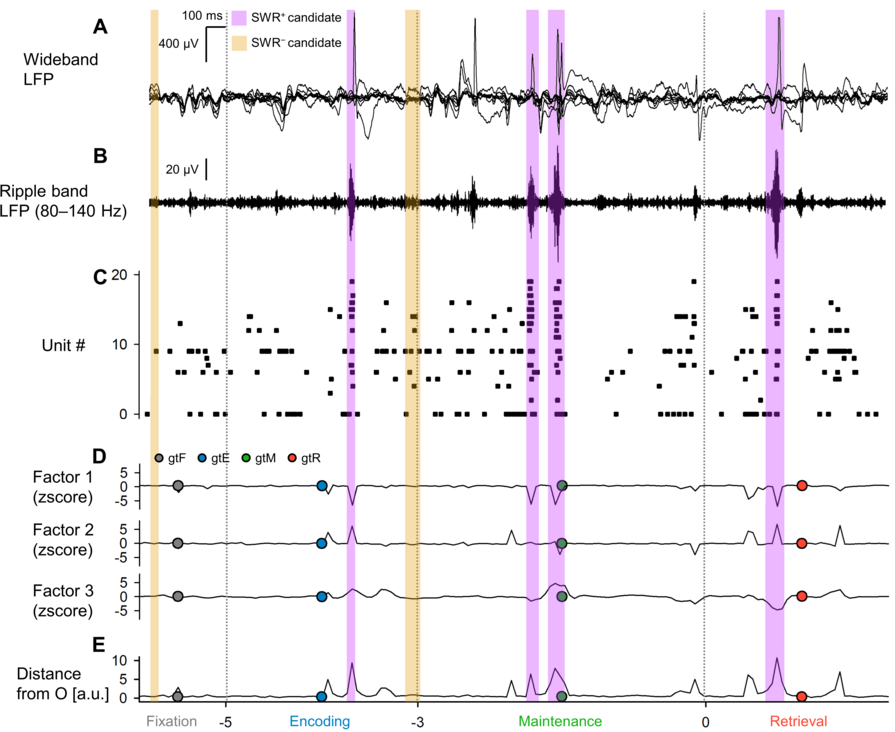
\includegraphics[width=1\textwidth]{./src/figures/.png/Figure_ID_01.png}
        	\caption{\textbf{
Local Field Potentials (LFP), Multiunit Activity, and Neural Trajectories in the Hippocampus During a Modified Sternberg Task
}
\smallskip
\\
\textbf{\textit{A.}} These traces show representative wideband LFP intracranial EEG (iEEG) signals recorded from the left hippocampal head. The subject performed a modified Sternberg working memory task, which includes fixation (1 s, \textit{gray}), encoding (2 s, \textit{blue}), maintenance (3 s, \textit{green}), and retrieval (2 s, \textit{red}). \textbf{\textit{B.}} We then present the corresponding ripple band LFP traces. \textbf{\textit{C.}} The raster plot depicts multiunit spikes taken from the LFP traces, sorted using a spike algorithm \cite{niediek_reliable_2016}. \textbf{\textit{D.}} Subsequently, we illustrate the neural trajectories, which are calculated by GPFA on spike counts per unit with 50-ms bins. Each phase's geometric median is marked by the dot circles. \textbf{\textit{E.}} The trajectory's distance from the origin $O$ is portrayed, with \textit{purple} and \textit{yellow} rectangles indicating the timings for SWR$^+$ candidates and SWR$^-$ candidates (considered as controls for SWR$^+$), respectively.
}
% width=1\textwidth
        	\label{fig:01}
        \end{figure*}
        \clearpage
        \begin{figure*}[ht]
            \pdfbookmark[2]{ID 02}{figure_id_02}
        	\centering
            \includegraphics[width=0.5\textwidth]{./src/figures/.png/Figure_ID_02.png}
        	\caption{\textbf{
State-Dependent Trajectories of Hippocampal Neurons
}
\smallskip
\\
\textbf{\textit{A.}} Neural trajectories within the initial three-dimensional factors derived from the Gaussian Process Factor Analysis (GPFA) are displayed. The smaller dots correspond to coordinates of 50-ms neural trajectory bins, while the larger dots with \textit{black} edges signify the geometric medians for respective stages in the Sternberg working memory task: fixation (\textit{gray}), encoding (\textit{blue}), maintenance (\textit{green}), and retrieval (\textit{red}). \textbf{\textit{B.}} The figure conveys the log-likelihood of the GPFA models versus the count of dimensions used to embed multiunit spikes found in the medial temporal lobe (MTL) territories. In specific, the elbow method pinpointed the optimal dimension to be three. \textbf{\textit{C.}} This panel illustrates the distance of the neural trajectories from the origin ($O$) for the hippocampus (Hipp.), entorhinal cortex (EC), and amygdala (Amy.), against the time elapsed from the probe onset. \textbf{\textit{D.}} The distance of the trajectory from $O$ within MTL regions is displayed. The hippocampus shows the farthest distance, followed by the EC and the Amygdala. \textbf{\textit{E.}} The plot represents inter-phase trajectory distances within the MTL regions.
Abbreviations:
}
% width=0.5\textwidth
        	\label{fig:02}
        \end{figure*}
        \clearpage
        \begin{figure*}[ht]
            \pdfbookmark[2]{ID 03}{figure_id_03}
        	\centering
            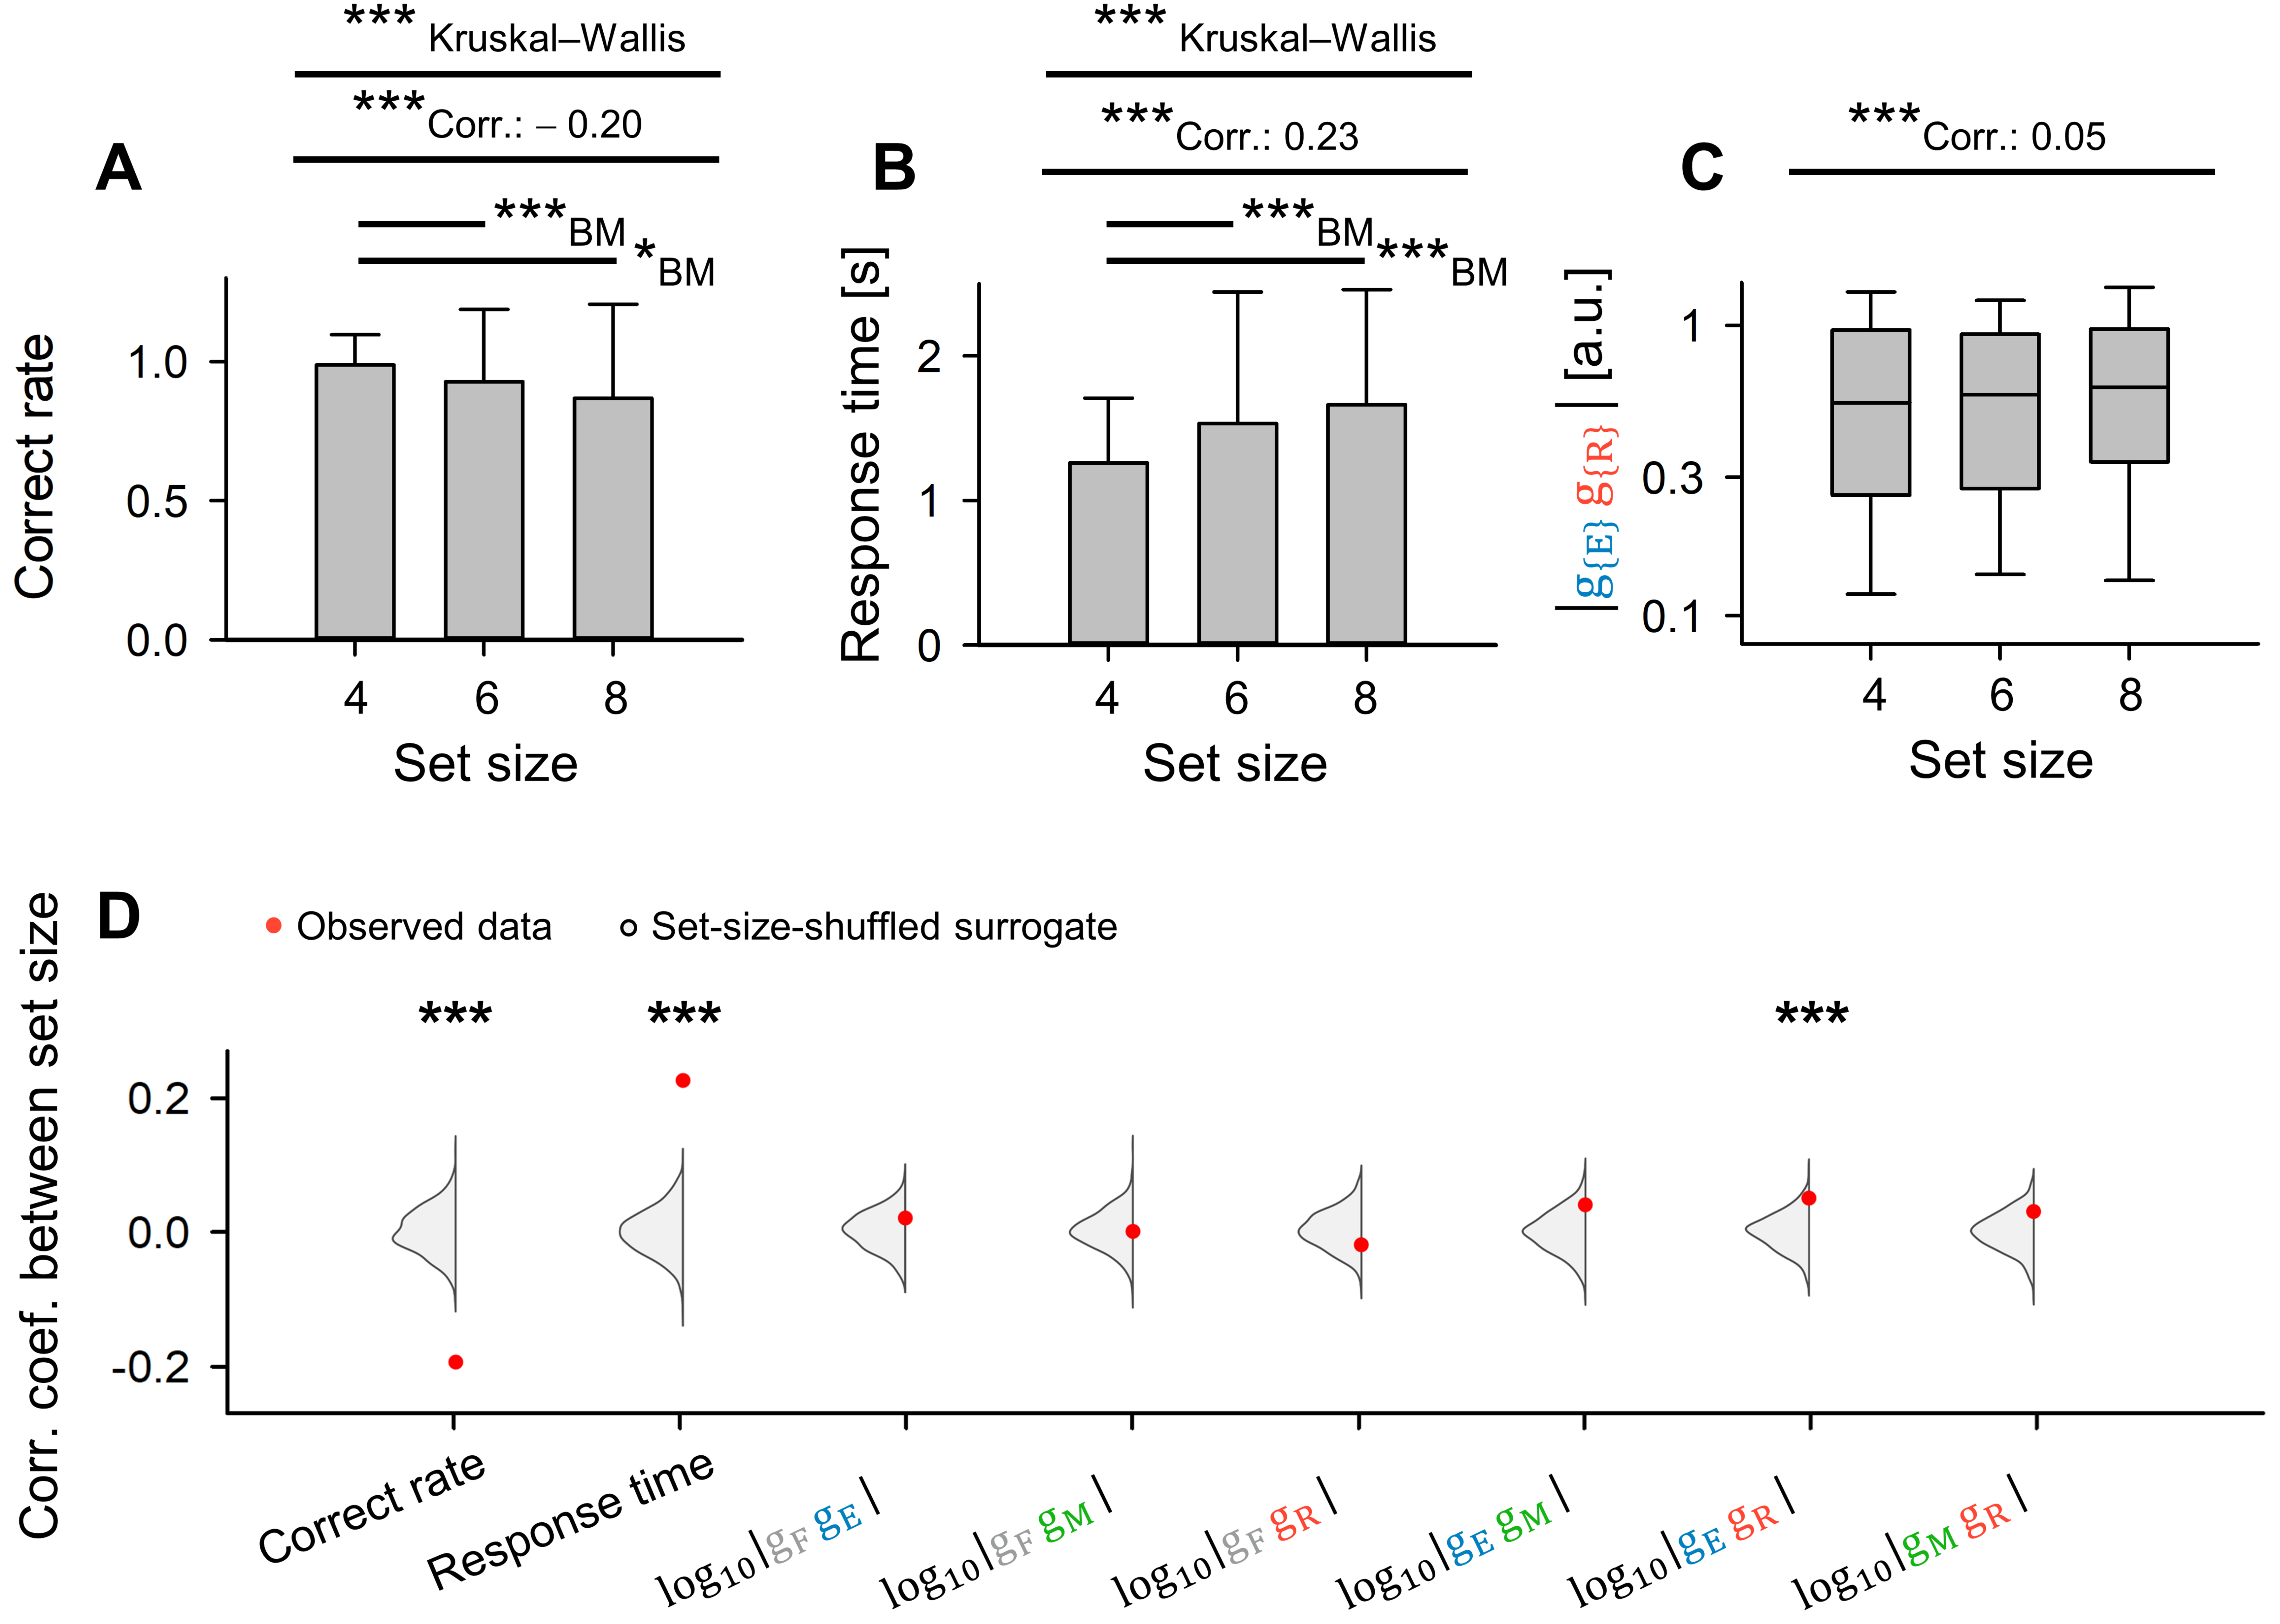
\includegraphics[width=1\textwidth]{./src/figures/.png/Figure_ID_03.png}
        	\caption{\textbf{
Dependency of Trajectory Distance on Memory Load: Encoding and Retrieval States in Hippocampus
}
\smallskip
\\
\textbf{\textit{A.}} The relationship between set size (number of letters that need to be encoded) and correct rate in the working memory task (coefficient = $-0.20$, ***\textit{p} $<$ 0.001). \textbf{\textit{B.}} The correlation between set size and response time (coefficient = 0.23, ***\textit{p} $<$ 0.001). \textbf{\textit{C.}} The impact of set size on the inter-phase distances between the encoding and retrieval phases ($\lVert \mathrm{g_{E}g_{R}} \rVert$) (correlation coefficient = 0.05). \textbf{\textit{D.}} \textit{Red} dots represent experimental observations of correlations between set size and the following parameters: correct rate, response time, $\log_{10}{\lVert \mathrm{g_{F}g_{E}} \rVert}$, $\log_{10}{\lVert \mathrm{g_{F}g_{M}} \rVert}$, $\log_{10}{\lVert \mathrm{g_{F}g_{R}} \rVert}$, $\log_{10}{\lVert \mathrm{g_{E}g_{M}} \rVert}$, $\log_{10}{\lVert \mathrm{g_{E}g_{R}} \rVert}$, and $\log_{10}{\lVert \mathrm{g_{M}g_{R}} \rVert}$. The \textit{gray} kernel density plot illustrates the corresponding set-size-shuffled surrogate (\textit{n} = 1,000) (***\textit{p}s $<$ 0.001).
}
% width=1\textwidth
        	\label{fig:03}
        \end{figure*}
        \clearpage
        \begin{figure*}[ht]
            \pdfbookmark[2]{ID 04}{figure_id_04}
        	\centering
            \includegraphics[width=1\textwidth]{./src/figures/.png/Figure_ID_04.png}
        	\caption{\textbf{
Detection of SWRs in Presumptive CA1 Regions
}
\smallskip
\\
\textbf{\textit{A.}} Two-dimensional UMAP (Uniform Manifold Approximation and Projection) \cite{mcinnes_umap_2018} projection of multiunit spikes during SWR$^+$ candidates (\textit{purple}) and SWR$^-$ candidates (\textit{yellow}). \textbf{\textit{B.}} Cumulative density plot shows silhouette scores, indicative of UMAP clustering quality, for hippocampal regions (see Table~\ref{tab:02} for reference). Note that hippocampal regions with silhouette scores greater than 0.60 (equivalent to the $75^{th}$ percentile) were identified as possible CA1 regions. SWR$^+$ and SWR$^-$ candidates recorded from these speculative CA1 regions were respectively classified as SWR$^+$ and SWR$^-$ (\textit{n}s = 1,170). \textbf{\textit{C.}} The identical distributions of durations are presented for SWR$^+$ (\textit{purple}) and SWR$^-$ (\textit{yellow}), owing to their definitions (93.0 [65.4] ms, median [IQR]). \textbf{\textit{D.}} SWR incidence for both SWR$^+$ (\textit{purple}) and SWR$^-$ (\textit{yellow}) obtained relative to the probe's timing is illustrated as a mean \textpm 95\% confidence interval. However, as the intervals may not be visible due to their narrow range, note that a significant increase in SWR incidence was detected during the initial 400 ms of the retrieval phase (0.421 [Hz], *\textit{p} $<$ 0.05, bootstrap test). \textbf{\textit{E.}} The distributions of ripple band peak amplitudes for SWR$^-$ (\textit{yellow}; 2.37 [0.33] SD of baseline, median [IQR]) and SWR$^+$ (\textit{purple}; 3.05 [0.85] SD of baseline, median [IQR]) are delineated (***\textit{p} $<$ 0.001, the Brunner--Munzel test).
}
% width=1\textwidth
        	\label{fig:04}
        \end{figure*}
        \clearpage
        \begin{figure*}[ht]
            \pdfbookmark[2]{ID 05}{figure_id_05}
        	\centering
            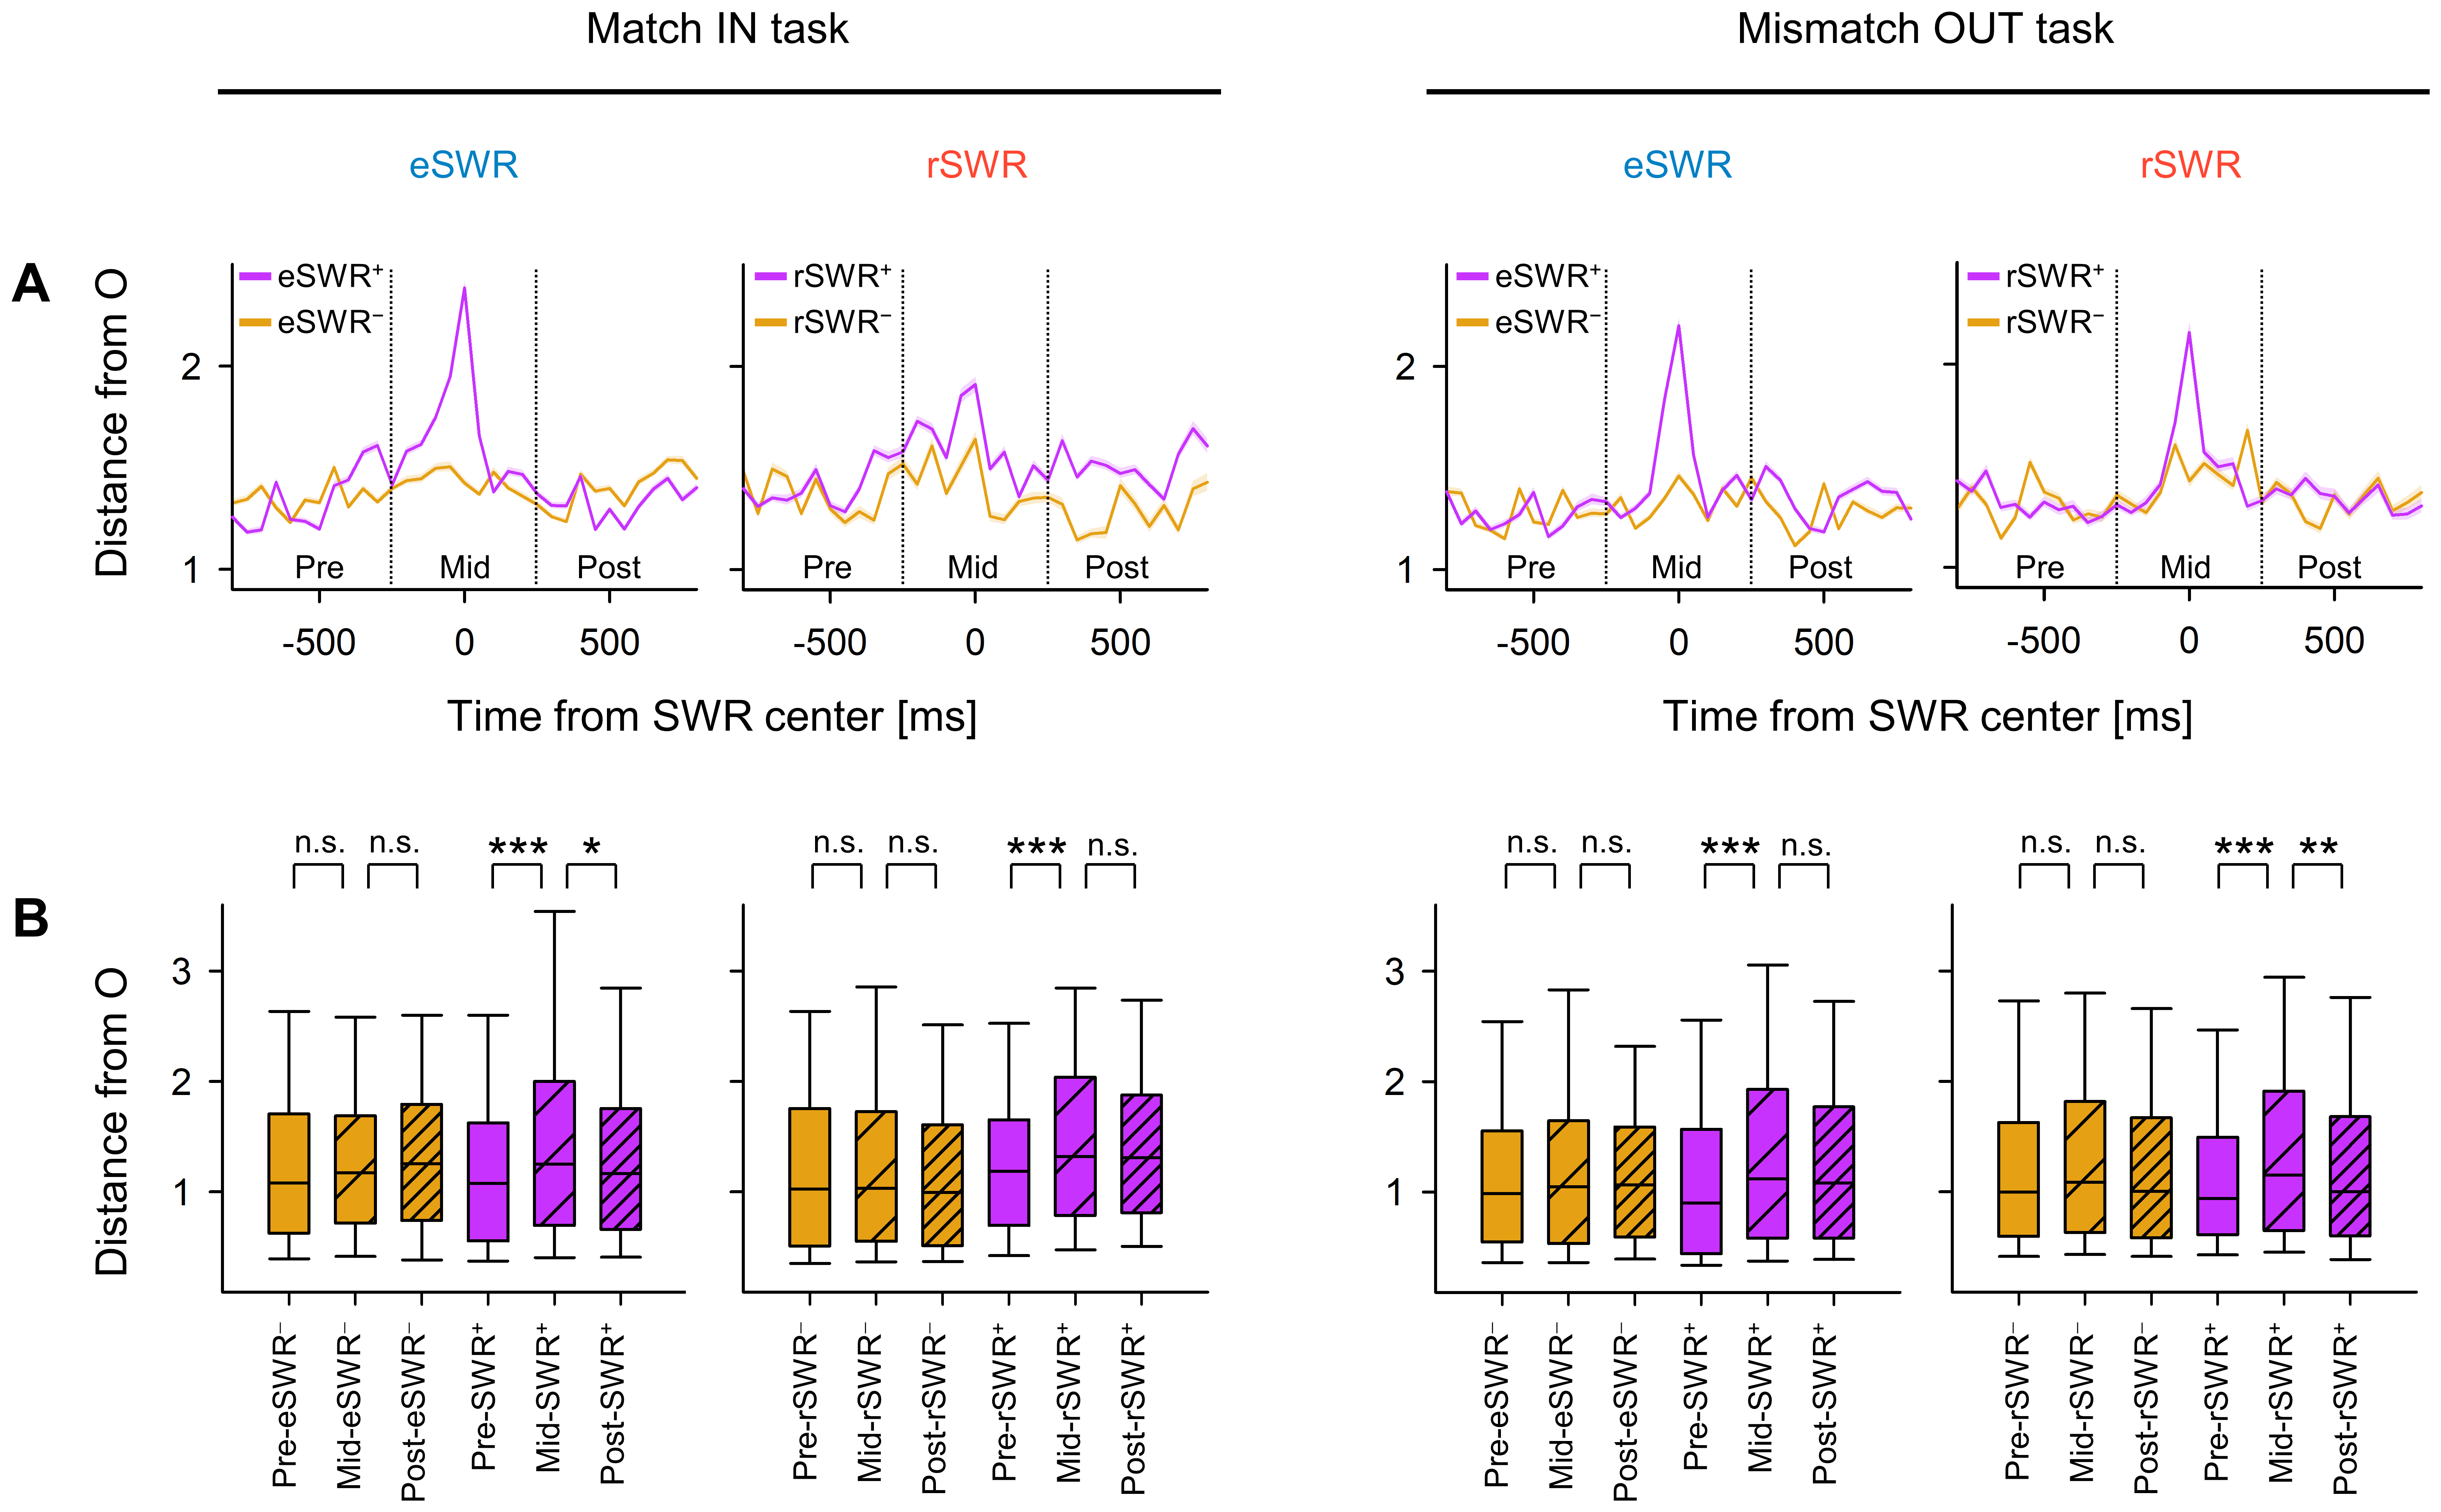
\includegraphics[width=1\textwidth]{./src/figures/.png/Figure_ID_05.png}
        	\caption{\textbf{
Transient Alterations in Neural Trajectory During SWR Events
}
\smallskip
\\
\textbf{\textit{A.}} Displayed is the distance from origin ($O$) of the peri-sharp-wave-ripple trajectory (mean \textpm 95\% confidence interval). The intervals may not be apparent due to their slender ranges. \textbf{\textit{B.}} Shown is the distance from the origin ($O$) during pre-, mid-, and post-SWR periods (*\textit{p} $<$ 0.05, **\textit{p} $<$ 0.01, ***\textit{p} $<$ 0.001; assessed using the Brunner--Munzel test). Abbreviations: SWR, sharp-wave ripple events; eSWR, SWR during the encoding phase; rSWR, SWR while in the retrieval phase; SWR$^+$, positive SWR event; SWR$^-$, control events for SWR$^+$; pre-, mid-, or post-SWR denote the time intervals from $-800$ to $-250$ ms, from $-250$ to $+250$ ms, or from $+250$ to $+800$ ms, all relative to the center of the SWR.
}
% width=1\textwidth
        	\label{fig:05}
        \end{figure*}
        \clearpage
        \begin{figure*}[ht]
            \pdfbookmark[2]{ID 06}{figure_id_06}
        	\centering
            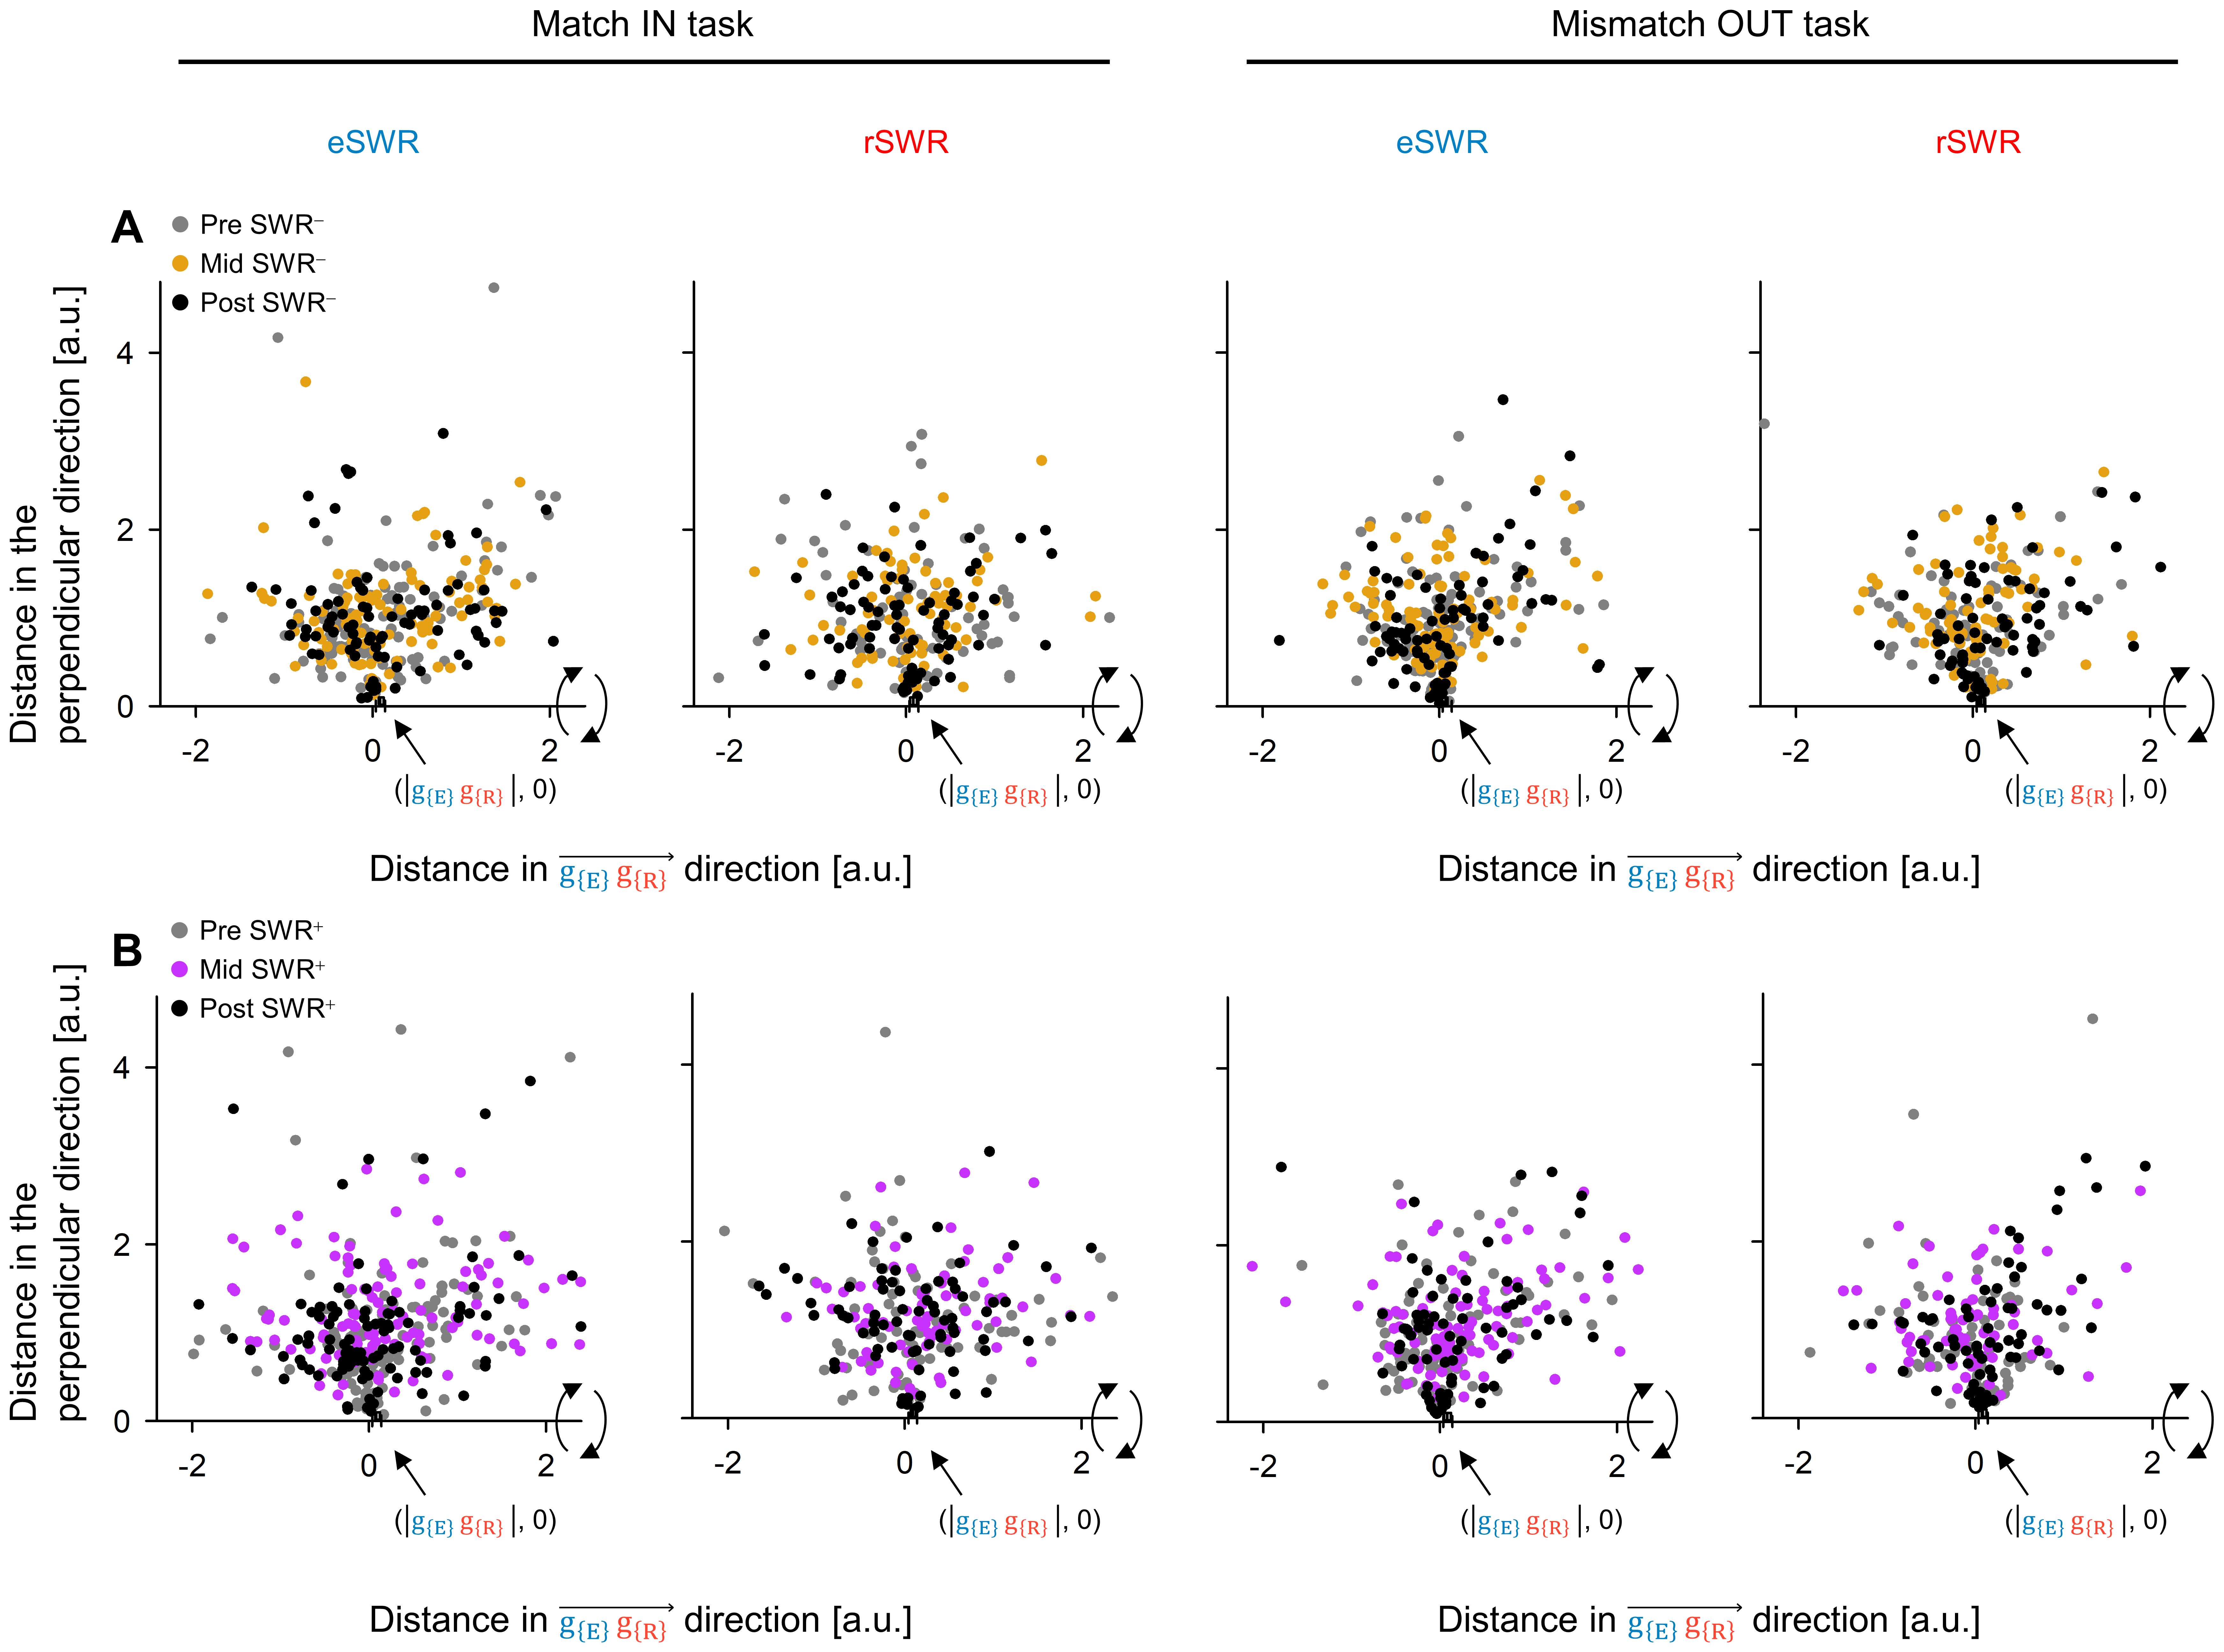
\includegraphics[width=1\textwidth]{./src/figures/.png/Figure_ID_06.png}
        	\caption{\textbf{
Visualization of Neural Trajectories during SWR in Two-Dimensional Spaces}
\smallskip
\\
The panels display hippocampal neural trajectories during SWR as projected onto two-dimensional spaces. \textbf{\textit{A.}} Indicates hippocampal neural trajectories pre-SWR$^-$ (\textit{gray}), mid-SWR$^-$ (\textit{yellow}), and post-SWR$^-$ (\textit{black}). \textbf{\textit{B.}} Represents the equivalents for SWR$^+$ as opposed to SWR$^-$. The $\lVert \mathrm{g_{E}g_{R}} \rVert$ varied among sessions. The projection was applied in the following manner: First, a linear transformation positioned $\mathrm{g_{E}}$ at the origin $O$ (0,0), and $\mathrm{g_{R}}$ at ($\lVert \mathrm{g_{E}g_{R}} \rVert$, 0). The point cloud was then rotated around the $\mathrm{g_{E}g_{R}}$ axis (equivalent to the x axis) for fitting into two-dimensional spaces. Therefore, within these two-dimensional spaces, both the distances from $O$ and the angles preserved the original makeup of the $\mathrm{g_{E}g_{R}}$ axis from the original three-dimensional spaces. Abbreviations: SWR signifies sharp-wave ripple events; eSWR denotes SWR during the encoding phase; rSWR indicates SWR during the retrieval phase; SWR$^+$, marks an SWR event; SWR$^-$ refers to control events for SWR$^+$; pre-SWR, mid-SWR, or post-SWR, reference the time intervals from $-800$ to $-250$ ms, from $-250$ to $+250$ ms, or from $+250$ to $+800$ ms from the center of SWR.
}
% width=1\textwidth
        	\label{fig:06}
        \end{figure*}
        \clearpage
        \begin{figure*}[ht]
            \pdfbookmark[2]{ID 07}{figure_id_07}
        	\centering
            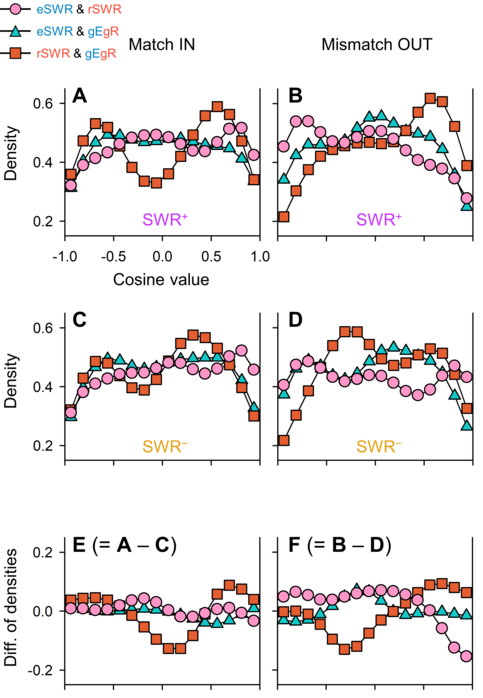
\includegraphics[width=0.5\textwidth]{./src/figures/.png/Figure_ID_07.png}
        	\caption{\textbf{
Directions of Neural Trajectories during SWRs Based on Encoding and Retrieval States
}
\smallskip
\\
\textbf{\textit{A--B}} Kernel density estimation (KDE) distributions of $\protect\overrightarrow{{\mathrm{eSWR^+}}} \cdot \protect\overrightarrow{{\mathrm{rSWR^+}}}$ (\textit{pink circles}), $\protect\overrightarrow{{\mathrm{eSWR^+}}} \cdot \protect\overrightarrow{{\mathrm{g_{E}g_{R}}}}$ (\textit{blue triangles}), and $\protect\overrightarrow{{\mathrm{rSWR^+}}} \cdot \protect\overrightarrow{{\mathrm{g_{E}g_{R}}}}$ (\textit{red rectangles}) in Match In (\textit{A}) and Mismatch OUT tasks (\textit{B}). \textbf{\textit{C--D}} Present the corresponding distributions of $\mathrm{SWR^-}$ instead of those of $\mathrm{SWR^+}$ in \textit{A} and \textit{B}. \textbf{\textit{E--F}} Depict the differences in the distributions of $\mathrm{SWR^+}$ and $\mathrm{SWR^-}$, illuminating the SWR components (\textit{E} = \textit{C} $-$ \textit{A}; \textit{F} = \textit{D} $-$ \textit{B}). Note the biphasic distributions of $\protect\overrightarrow{{\mathrm{rSWR^-}}} \cdot \protect\overrightarrow{{\mathrm{g_{E}g_{R}}}}$, suggesting fluctuations between the encoding and retrieval states during the Sternberg task. Moreover, inverse directionality between $\protect\overrightarrow{{\mathrm{eSWR^+}}}$ and $\protect\overrightarrow{{\mathrm{rSWR^+}}}$ was observed (\textit{pink circles}) in the Mismatch OUT task, but not in the Match IN task \textbf{\textit{E--F}}). Finally, shifts from the retrieval to encoding states were evident in the SWR components in both the Match IN and Mismatch OUT tasks (\textit{red rectangles} in \textit{E} and \textit{F}).
}
% width=0.5\textwidth
        	\label{fig:07}
        \end{figure*}

%%%%%%%%%%%%%%%%%%%%%%%%%%%%%%%%%%%%%%%%%%%%%%%%%%%%%%%%%%%%%%%%%%%%%%%%%%%%%%%%
%% END
%%%%%%%%%%%%%%%%%%%%%%%%%%%%%%%%%%%%%%%%%%%%%%%%%%%%%%%%%%%%%%%%%%%%%%%%%%%%%%%%

\end{document}
